\documentclass{article}

\usepackage{titlesec}
\usepackage{longtable}
\usepackage{array} % for defining a new column type
\usepackage{varwidth} %for the varwidth minipage environment
\usepackage{color, colortbl}
\usepackage{caption}
\usepackage{subfigure}
\usepackage{filecontents}
\usepackage[section]{placeins}
\usepackage{float}

\definecolor{Gray}{gray}{0.9}

\usepackage{pgf-umlsd}
\usepackage{pgf-umlcd}
\newcommand{\sectionbreak}{\clearpage}

\begin{document}

\newcolumntype{M}{>{\begin{varwidth}{4cm}}l<{\end{varwidth}}} %M is for Maximal column

\begin{titlepage}
	\Huge{Assignment 1}
\end{titlepage}


\section{The Core}

\subsection{Derive Classes}
For deriving the the right classes that we can implement in the software we firstly look for noun phrases in the requirements document\footnote{https://github.com/mkhattat/bitcode-SEM/blob/master/docs/requirements.pdf}. Secondly we try to refine the list of phrases and group them by using given guidelines.

\paragraph{Noun phrases}
In table \ref{table:ListDerivedNouns} a list of noun phrases is presented that was derived from the functional requirements in the requirements document.

\begin{center}
    \begin{longtable}{ | p{1in} | p{3in} |}
    \hline
    \rowcolor{Gray}
    Noun Phrases & Requirement \\ \hline
    game, board, grid & The game board will consist of a 10x10 square grid \\ \hline
    tile & The game will have six different tiles with which the board will be filled.\\ \hline
    filled board & The game will start with a filled board.\\ \hline
    mouse & A tile must be able to move horizontal or vertical by using the mouse.\\ \hline
    row, column & If one tile is moved, the whole row or column will move along with it. The tiles that get past the edge will reappear at the opposite edge. \\ \hline
	... & A row or column of 3 or more of the same tile (independent of the white outline), will mean that these tiles get removed from the game. \\ \hline
	... & The tiles above empty tiles will move down one position, the remaining empty tiles shall be filled randomly. \\ \hline
	player, move & The game will end when the player runs out of possible moves. \\ \hline
	... & The player should be able to start a new game. \\ \hline
	... & The player should be able to stop a game in progress. \\ \hline
	... & The game shall end when the player loses or stops the game, or clears all of the white outlining. \\ \hline
	turn, cell & The game will end in a set amount of turns. The amount is based upon the amount of cells which are outlined. (For example 1 outlined cell gives the player five moves). \\ \hline
	white outline & Some cells will have a white outline, moving the tile which rests on this cell will not affect the white outline. \\ \hline
	... & The white outlining of a cell will be removed once a tile in that cell is removed. \\ \hline
	pattern & The patterning of white tiles should be preprogrammed. \\ \hline
	... & The player loses when there are no possible moves left, or if the player has run out of moves. \\ \hline
	... & The player wins when all white outlined cells are cleared. \\ \hline
	level, difficulty system & The game could have a level or difficulty based system. \\ \hline
	scoring system & The game could have a scoring system based on the level or difficulty system. \\ \hline
	score & The players score could be shown during the game. \\ \hline
	\caption{list of derived nouns}\label{table:ListDerivedNouns}
    \end{longtable}
\end{center}


\paragraph{Refine Candidates} We can refine the list of nouns by sorting them based on the groups of obvious, uncertain or nonsense class candidates. We also define the type of candidate classes such that it can be a physical object, conceptual entity, categories of classes an interface or values. In table \ref{table:ListCandidateClasses} a list of candidate classes is shown.

\begin{center}
    \begin{longtable}{ | p{1in} | p{1in} | p{2in} |}
    \hline
    \rowcolor{Gray}
    Candidate Class & Group & Class Type \\ \hline
	Game & obvious & conceptual entity \\ \hline
	Board & obvious & interface \\ \hline
	Tile & obvious & conceptual entity \\ \hline
	Mouse & obvious & physical object \\ \hline
	Player & obvious & physical object \\ \hline
	Level & obvious & conceptual entity \\ \hline
	Grid & uncertain & value \\ \hline
	Move & uncertain & conceptual entity \\ \hline
	Pattern & uncertain & value \\ \hline
	ScoringSystem & uncertain & conceptual entity \\ \hline
	Score & uncertain & conceptual entity \\ \hline
	FilledBoard & nonsense & conceptual entity \\ \hline
	Row, Column & nonsense & conceptual entity \\ \hline
	Turn & nonsense & conceptual entity \\ \hline
	WhiteOutline & nonsense & conceptual entity \\ \hline

	\caption{list of candidate classes}\label{table:ListCandidateClasses}
    \end{longtable}
\end{center}


\paragraph{Class-Responsibility-Collaboration Cards} After we refined the list of candidate classes we can create so called "class-responsibility-collaboration Cards" or CRC cards. These cards are used to get an overview of the responsibility of the classes and which classes are collaborating together. In the figure below the CRC cards are presented.

%\documentclass{article}\usepackage{subfigure}\usepackage{float}\begin{document}

\begin{figure}[H]
\begin{subfigure}{}
		\begin{tabular}{|p{1in}|p{1in}|}
			\hline
			\multicolumn{2}{|p{2in}|}{\textbf{Game}} \\ \hline
			\multicolumn{2}{|p{2in}|}{Supperclass(es): ...} \\ \hline
			\multicolumn{2}{|p{2in}|}{Subclasses: ...} \\ \hline
			Create game window	& ... \\ \hline
			Create board & Board \\ \hline
			Create player & Player \\ \hline
		\end{tabular}
		\begin{tabular}{|p{1in}|p{1in}|}
			\hline
			\multicolumn{2}{|p{2in}|}{\textbf{Board}} \\ \hline
			\multicolumn{2}{|p{2in}|}{Supperclass(es): ...} \\ \hline
			\multicolumn{2}{|p{2in}|}{Subclasses: ...} \\ \hline
			Read level & Level \\ \hline
			Create grid & Grid \\ \hline
			Draw board & Tile \\ \hline
			Move Tiles & Move \\ \hline
		\end{tabular}
\end{subfigure}
\begin{subfigure}{}
		\begin{tabular}{|p{1in}|p{1in}|}
			\hline
			\multicolumn{2}{|p{2in}|}{\textbf{Tile}} \\ \hline
			\multicolumn{2}{|p{2in}|}{Supperclass(es): ...} \\ \hline
			\multicolumn{2}{|p{2in}|}{Subclasses: ...} \\ \hline
			Load Image & ... \\ \hline
			Draw Tile & ... \\ \hline
		\end{tabular}
		\begin{tabular}{|p{1in}|p{1in}|}
			\hline
			\multicolumn{2}{|p{2in}|}{\textbf{Move}} \\ \hline
			\multicolumn{2}{|p{2in}|}{Supperclass(es): ...} \\ \hline
			\multicolumn{2}{|p{2in}|}{Subclasses: ...} \\ \hline
			Check for movements & EventHandler \\ \hline
			Move animation & Tile, Grid \\ \hline
		\end{tabular}
\end{subfigure}
\begin{subfigure}{}
		\begin{tabular}{|p{1in}|p{1in}|}
			\hline
			\multicolumn{2}{|p{2in}|}{\textbf{EventHandler}} \\ \hline
			\multicolumn{2}{|p{2in}|}{Supperclass(es): ...} \\ \hline
			\multicolumn{2}{|p{2in}|}{Subclasses: ...} \\ \hline
			Check for mouse events & MouseEvent Handler \\ \hline
			Check for button events & ButtonEvent Handler \\ \hline
		\end{tabular}
		\begin{tabular}{|p{1in}|p{1in}|}
			\hline
			\multicolumn{2}{|p{2in}|}{\textbf{Player}} \\ \hline
			\multicolumn{2}{|p{2in}|}{Supperclass(es): ...} \\ \hline
			\multicolumn{2}{|p{2in}|}{Subclasses: ...} \\ \hline
			keep track of score & ScoringSystem \\ \hline
		\end{tabular}
\end{subfigure}
\begin{subfigure}{}
		\begin{tabular}{|p{1in}|p{1in}|}
			\hline
			\multicolumn{2}{|p{2in}|}{\textbf{MouseEventHandler}} \\ \hline
			\multicolumn{2}{|p{2in}|}{Supperclass(es): ...} \\ \hline
			\multicolumn{2}{|p{2in}|}{Subclasses: ...} \\ \hline
			Capture and handle mouse events & ... \\ \hline
		\end{tabular}
		\begin{tabular}{|p{1in}|p{1in}|}
			\hline
			\multicolumn{2}{|p{2in}|}{\textbf{ButtonEventHandler}} \\ \hline
			\multicolumn{2}{|p{2in}|}{Supperclass(es): ...} \\ \hline
			\multicolumn{2}{|p{2in}|}{Subclasses: ...} \\ \hline
			Capture and handle button events & ... \\ \hline
		\end{tabular}
\end{subfigure}
\begin{subfigure}{}		
		\begin{tabular}{|p{1in}|p{1in}|}
			\hline
			\multicolumn{2}{|p{2in}|}{\textbf{ScoringSystem}} \\ \hline
			\multicolumn{2}{|p{2in}|}{Supperclass(es): ...} \\ \hline
			\multicolumn{2}{|p{2in}|}{Subclasses: ...} \\ \hline
			Keep track of scoring & Move \\ \hline
		\end{tabular}
		\begin{tabular}{|p{1in}|p{1in}|}
			\hline
			\multicolumn{2}{|p{2in}|}{\textbf{Level}} \\ \hline
			\multicolumn{2}{|p{2in}|}{Supperclass(es): ...} \\ \hline
			\multicolumn{2}{|p{2in}|}{Subclasses: ...} \\ \hline
			Read Level from file & ... \\ \hline
		\end{tabular}
\end{subfigure}

\end{figure}
%\end{document}

\paragraph{Comparison with the implementation} If we look at classes that were integrated into the initial implementation of the game\footnote{https://github.com/mkhattat/bitcode-SEM/releases} we can spot some differences. Namely, there are a couple of classes missing. This is mostly due to the fact that not all requirements where implemented in the initial version. For example, the Player class and the ScoringSystem class is absence from the code because scoring is not implemented. There is also not a Level class because there exists only one level that is randomly generated. Furthermore, the Game class is replaced by the Launcher class and Move class is replaced by the Animation class.


\subsection{Main Classes}
text

\subsection{Reflect on main class decisions}
text

\subsection{The Class diagram}
text

\subsection{The Sequence Diagram}
	\begin{figure}[H]
		\centering
		\begin{sequencediagram}
			\newthread{A}{User}{}
			\newthread{B}{Window/EventHandler}{}
			\newthread{C}{Game}{}
			\newthread{D}{Board}{}
			\begin{call}{A}{Drag Item}{B}{}
				\begin{call}{B}{Check for triples}{C}{}
					\begin{call}{C}{Check for triples}{D}{}
						\begin{sdblock}{Recursion}{}
							\begin{call}{D}{Check for triples}{D}{}
							\end{call}
						\end{sdblock}
					\end{call}
				\end{call}
			\end{call}
		\end{sequencediagram}
	\end{figure}



\section{UML in Practice}
text

\subsection{Composition and Aggregation}
text

\subsection{Parametrized Classes}
text

\subsection{Hierarchy Class Diagrams}
\centering
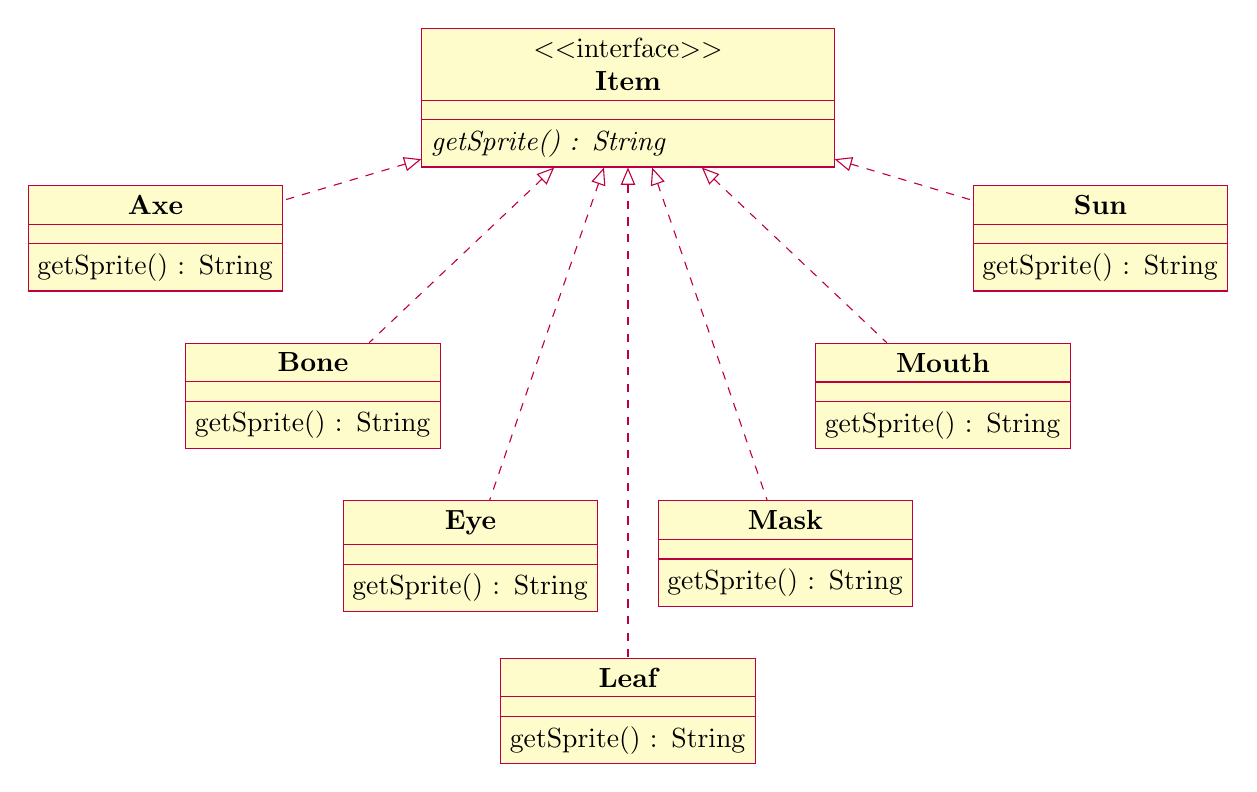
\begin{tikzpicture}
\begin{interface}{Item}{0,0}
\operation[0]{getSprite() : String}
\end{interface}
\begin{class}[text width = 3cm]{Axe}{-6,-2}
\implement{Item}
\operation{getSprite() : String}
\end{class}
\begin{class}[text width = 3cm]{Bone}{-4,-4}
\implement{Item}
\operation{getSprite() : String}
\end{class}
\begin{class}[text width = 3cm]{Eye}{-2,-6}
\implement{Item}
\operation{getSprite() : String}
\end{class}
\begin{class}[text width = 3cm]{Leaf}{0,-8}
\implement{Item}
\operation{getSprite() : String}
\end{class}
\begin{class}[text width = 3cm]{Mask}{2,-6}
\implement{Item}
\operation{getSprite() : String}
\end{class}
\begin{class}[text width = 3cm]{Mouth}{4,-4}
\implement{Item}
\operation{getSprite() : String}
\end{class}
\begin{class}[text width = 3cm]{Sun}{6,-2}
\implement{Item}
\operation{getSprite() : String}
\end{class}
\end{tikzpicture}

Items are produced by an item factory, which can create each of the seven types of items.
Each item implements the item interface, as a result the board can contain every type of item and request its sprite.
A similar functionality could be implemented using an item class with an id attribute, however such an implementation would make further expanding each item individually much more complicated and inconvenient.




\end{document}

